\documentclass[12pt,a4paper]{article}
\usepackage [french]{babel}
\usepackage [utf8]{inputenc}
\usepackage [T1] {fontenc}
\linespread{1.6}

\usepackage{indentfirst}
\usepackage{graphicx}
\usepackage{ragged2e}
\usepackage{blindtext}
\usepackage{lmodern}
\usepackage[table]{xcolor}
\usepackage{diagbox}
\usepackage{multirow}
\usepackage{wrapfig, calc}
\usepackage{fancyhdr}
\pagestyle{fancy}
\usepackage{pdfpages}
\usepackage{afterpage}
\input{insbox}

%\addtolength{\oddsidemargin}{-.5in}
%\addtolength{\evensidemargin}{-.5in}
%\addtolength{\textwidth}{1in}
%\addtolength{\topmargin}{-.5in}
%\addtolength{\textheight}{1in}

%-------------------------------------


\begin{document}
\renewcommand{\headrulewidth}{1pt}
\fancyhead[L]{
%
\includegraphics[scale=0.02]{images/logo-epita-nb.jpg}

\includegraphics[scale=0.01]{images/Epita.png}
}
\fancyhead[R]{\leftmark}

\renewcommand{\footrulewidth}{1pt}
\fancyfoot[R]{page \thepage} 
\fancyfoot[C]{Cahier des charges - \textbf{Animatch}}



\begin{titlepage}
\linespread{1}


\begin{center}

\huge Cahier des charges
\begin{center}
\rule{0.5\linewidth}{1pt}
\end{center}
\huge \textbf{Animatch}\\
\vspace{48pt}
%
\includegraphics[width = 0.8\textwidth]{images/logo-epita-nb.jpg}

\includegraphics[width = 0.8\textwidth]{images/Epita.png}
\centering\\
\vspace{48pt}
\large ILLUSION \\
\vspace{12pt}
Adrien Coureau\\
Josselin Priet\\
Guillaume Rat\\
Hector Thubert \\
Guilhem Dardonville\\
\vspace{36pt}
Date d'échéance : 26 octobre 2023 \\

\end{center}

\end{titlepage}
\linespread{1.6}

\setcounter{page}{0}
\tableofcontents
\clearpage

\section{Introduction}
\textbf{Animatch} est le tout premier produit de l'entreprise indépendante ILLUSION. Animatch est un jeu de duel stratégique et de création de deck à destruction de terrain dans lequel deux joueurs s'affrontent. Il sera disponible sur la plateforme Windows mais une déportation vers Android et iOS est également possible. 

Le jeu est en deux dimensions, et chaque joueur prend tour à tour le contrôle d'un groupe d'animaux dont l'objectif est d'éliminer le groupe adverse. Pour ce faire, avant le début de la partie, chaque joueur construit son propre deck de cartes, qu'il va pouvoir débloquer progressivement au cours de son expérience sur le jeu.

Chaque carte représente une action qui a un coût associé au coût de la carte. Les cartes sont utilisées pour éliminer les animaux adverses (par des tirs de missiles, des coups au corps-à-corps, etc...), pour détruire le terrain, pour faire tomber son adversaire dans le vide, ou encore pour se déplacer, ce qui offre des possibilités infinies de stratégies à l'utilisateur. Une partie se termine lorsque l'un des deux joueurs a réussi à éliminer le groupe d'animaux adverse.

En somme, Animatch peut être rapproché d'un mélange entre le jeu \textit{Worms} (1995) et le jeu \textit{Clash Royale} (2016). Il est accessible à tout public, amusant, et surtout, divertissant. Le multijoueur sera donc basé sur du "Matchmaking", un mécanisme de formation automatique de partie. Un joueur appuie sur le bouton pour jouer puis attend qu'un autre joueur le fasse aussi, ils entrent alors dans la partie et se retrouvent l'un contre l'autre.

Le jeu sera également doté d'une intelligence artificielle que l'utilisateur pourra affronter s'il décide de jouer seul. Celle-ci aura la capacité de faire des coups stratégiques pour battre le joueur. Le bot se formera une intelligence à la fois par le choix des cartes jouées, par la position des actions (combat), et par le calcul des trajectoires ("Path Finder") afin d'évaluer les gains et les pertes grâce à un algorithme poussé.

La création de ce produit permet de faire acquérir de nombreuses compétences informatiques utiles à de futurs ingénieurs en informatique, membres du groupe de travail, mais aussi de créer un contenu ludique et amusant, réutilisable de multiples fois.

Animatch sera créé de zéro et intégralement par notre équipe en utilisant un moteur de jeu open source. Ainsi, le budget de l'entreprise est de 0€ et aucune ressource ne sera achetée au cours de la création. Le code, les graphismes, le son et la musique seront entièrement réalisés par l'entreprise.

Ce cahier des charges sert à expliquer comment le jeu sera construit jusqu'à sa phase finale, depuis les concepts qui définissent le jeu jusqu'aux rôles de chaque membre de l'équipe. Il évoquera aussi les étapes et la planification du calendrier afin de respecter l'échéance souhaitée par l'école EPITA.
\clearpage

\section{Cahier des charges fonctionnel}

\subsection{Origine et nature du projet}
Pour que notre projet se déroule avec le moins d'obstacles possible et que nous soyons enthousiastes à l'idée de travailler dessus, il était important d'être tous d'accord sur le type de jeu que nous allions développer. En posant la question au sein de notre groupe, nous sommes parvenus à un accord sur un jeu à partir de jeux de cartes.

Après avoir recueilli l'avis de l'ensemble des membres de notre entreprise, nous avons statué sur un mélange de deux types de jeux. Le jeu se reportera donc sur un style tactique en "deckbuilding" (jeux de cartes), où l'importance de la création d'un deck équilibré entre les différentes notions que comportera le jeu est primordiale afin de battre l'adversaire. Le déroulement de la partie fonctionne sur le principe de combat en tour par tour. L'idée serait que chacun joue ses tours sans que l'adversaire puisse répondre afin de créer une mécanique de jeu stratégique et intéressante, dépendante du placement du joueur et de ses capacités pour effectuer (ou pas) des actions. Cela crée alors une diversité conséquente de choix, qui dépendrait du deck créé au préalable.

Ce mélange de caractéristiques de jeux nous permettra de créer une dimension stratégique au jeu nécessaire afin que chaque joueur puisse acquérir un niveau plus élevé dans le jeu. Pour créer des decks optimisés, il faudra prendre en compte que les cartes ne sont pas toutes débloquées dès le départ ; il faudra les débloquer au fur et à mesure. Plus l'utilisateur jouera, plus il aura de possibilités pour complexifier son deck.
\clearpage


\subsection{Objet de l'étude}
L'entreprise s'est fixée pour objectif majeur de développer un jeu extrêmement divertissant, conçu pour captiver une grande variété de joueurs, quel que soit leur âge. L'ambition est de transformer chaque instant de jeu, partagé entre amis, en famille ou même seul (avec l'intelligence artificielle) en une expérience ludique et stratégique. Si c'est possible, le projet sera même déporté sur téléphone pour permettre au joueur de s'amuser dans toutes circonstances.

À travers ce projet, l'entreprise a l'intention de mettre en avant ses compétences en matière de créativité et de complexité, en témoignant d'un travail collaboratif efficace. Animatch constituera une véritable stimulation pour les joueurs, pouvant même devenir un jeu addictif, les poussant à élaborer des stratégies ingénieuses et à exercer leur réflexion pour parvenir à la victoire. 

L'élaboration du jeu Animatch, s'il permet de divertir les joueurs, démontrera également la capacité de notre entreprise à travailler en équipe pour aboutir à un projet concret de jeu vidéo. A titre individuel, cette conception permettra à chaque membre d'apprendre le travail collectif , de se dépasser pour atteindre la qualité, et de se perfectionner en apprenant à utiliser Notion ou des plate-formes de partage de fichiers comme GitLab ou GitHub.
\clearpage

\subsection{État de l'art}
Animatch représente un mélange de plusieurs genres de jeux distincts. Trouver un jeu au style identique est donc très compliqué. Cependant, notre concept de base a été inspiré par le jeu \textit{Worms} (1995) développé par Team17. L'idée d'un affrontement entre deux camps, avec un terrain destructible et de nombreuses possibilités de combat (avec des stratégies adaptables en fonction des choix de mouvement, d'attaque ou de dissimulation) forme la base de notre projet qui a suscité l'enthousiasme de tous.

Notre intention était de ne pas se limiter à un seul genre de jeu, mais plutôt de créer un mélange stratégique alliant divertissement et complexité tactique. Notre concept stratégique s'articule autour de la création de decks, similaire à \textit{Clash Royale} (2016) ou \textit{Hearthstone} (2014), permettant aux joueurs de choisir le style de jeu qu'ils souhaitent développer. Ainsi, un joueur peut opter pour un deck orienté vers l'offensive, axé sur la mobilité ou pour un deck défensif, selon ses préférences.

À cela s'ajoute un élément de collection : les cartes ne sont pas toutes débloquées au début, et il faudra les récupérer en jouant, permettant ainsi aux joueurs de progresser, au fil du temps, dans le jeu. Notre approche de la collection s'inspire du modèle de \textit{Clash Royale}. Plus les joueurs s'investissent, plus ils accumulent des récompenses, ce qui leur permet d'améliorer, de débloquer et finalement d'utiliser différentes cartes.

Dans notre projet nous nous inspirons du concept de \textit{Clash Royale}. Ce jeu a été lancé en 2016 sur les plate-formes mobiles, telles que les téléphones et les tablettes. Le succès de ce jeu, développé par une entreprise déjà renommée dans le monde du jeu mobile (Supercell), réside dans son système de jeu unique. L'acquisition progressive de cartes, le passage d'arène en arène au fur et à mesure des victoires, procure aux joueurs une satisfaction qui les incite à continuer à jouer. En suivant ce principe, Supercell a régulièrement mis à jour le jeu en ajoutant de nouvelles cartes, arènes et compétitions, ce qui a permis de fidéliser un grand nombre de joueurs. Même après sept ans d'existence, le jeu continue de fonctionner avec succès. C'est sur ce modèle similaire que nous avons l'intention de développer Animatch, en mettant l'accent sur le système de cartes, notamment au début de l'expérience de jeu.

Animatch s'inspirerait aussi de 2 grands axes de \textit{Worms}: l'idée du duel en 2D et celle d'un terrain destructible. \textit{Worms} doit en effet son succès à son style de combat qui, pour l'époque, en 1995, changeait beaucoup par rapport aux jeux vidéo classiques. De plus, il se démarque par l'option de détruire le terrain (grâce au lancers de grenade, de lance-roquettes ou autres),  qui faisait et fait toujours le charme du jeu. C'est donc ces 2 principales idées que Animatch prendrait en compte afin de créer un gameplay amusant et différent des jeux déjà existants.
\clearpage

\subsection{L'entreprise}
Fondée au début du mois d'octobre au cours d'une session en sciences humaines, ILLUSION a vu le jour grâce à la détermination de deux membres fondateurs, M. Coureau et M. Priet. La vision partagée par ces membres a ensuite attiré l'expertise de M. Thubert, M. Rat et M. Dardonville, qui ont rejoint le projet avec enthousiasme.

ILLUSION est composée de cinq membres entièrement investis dans la réussite de cette entreprise. Chacun d'entre eux apporte une contribution unique à l'équipe, combinant leurs compétences et leur passion. Cette unité et cette diversité de talents sont les fondements sur lesquels repose ILLUSION et sont ce qui mènera ce projet à la réussite.

L'entreprise tire son nom de la capacité des jeux vidéo à créer une ILLUSION d'immersion totale pour le joueur, l'amenant à croire qu'il se trouve réellement dans un monde fictif. Le choix de ce nom a été déterminé à la suite d'un vote des membres de l'entreprise.

ILLUSION se spécialise dans le développement de jeux vidéo et utilise une combinaison de logiciels pour mener à bien son premier projet. L'entreprise s'appuie sur Notion pour centraliser, stocker et organiser les données, et Discord pour communiquer simplement. Elle utilise le moteur de jeu Godot, qui est open-source et en constante évolution depuis plusieurs années. Ce moteur offre des capacités de développement en langage C\#, et est optimal pour le rendu 2D et pour le calcul des éléments de physique et pour la création d'animations nécessaires à la conception d'un jeu.

ILLUSION n'a pas encore conçu de projet, celui ci est le premier et l'équipe mettra tout en œuvre pour le concrétiser avec succès.

\clearpage

\subsection{L'équipe} 

\InsertBoxR{0}{
\includegraphics[scale=0.03]{images/adrien.coureau.jpg}}
Adrien, chef de projet, 18 ans, actuellement élève à EPITA, passionné d'informatique depuis petit. L'univers de la création l'attire beaucoup (dessin, sculpture, dessin digital, production de musique). Il a commencé à créer ses premiers jeux avec Scratch puis Python en 5ème, puis en terminale un jeu de A à Z en Pygame (code, art, son), ce qui l'a ensuite amené à prendre cette voie dans laquelle il souhaite exprimer sa créativité.

\noindent Dans ce projet, Adrien sera utile pour la conception théorique (équilibrage du jeu), la conception graphique et sonore, et la programmation. Il saura aussi mener à bien le travail collectif de l'équipe en tant que chef de projet.\\

\InsertBoxL{0}{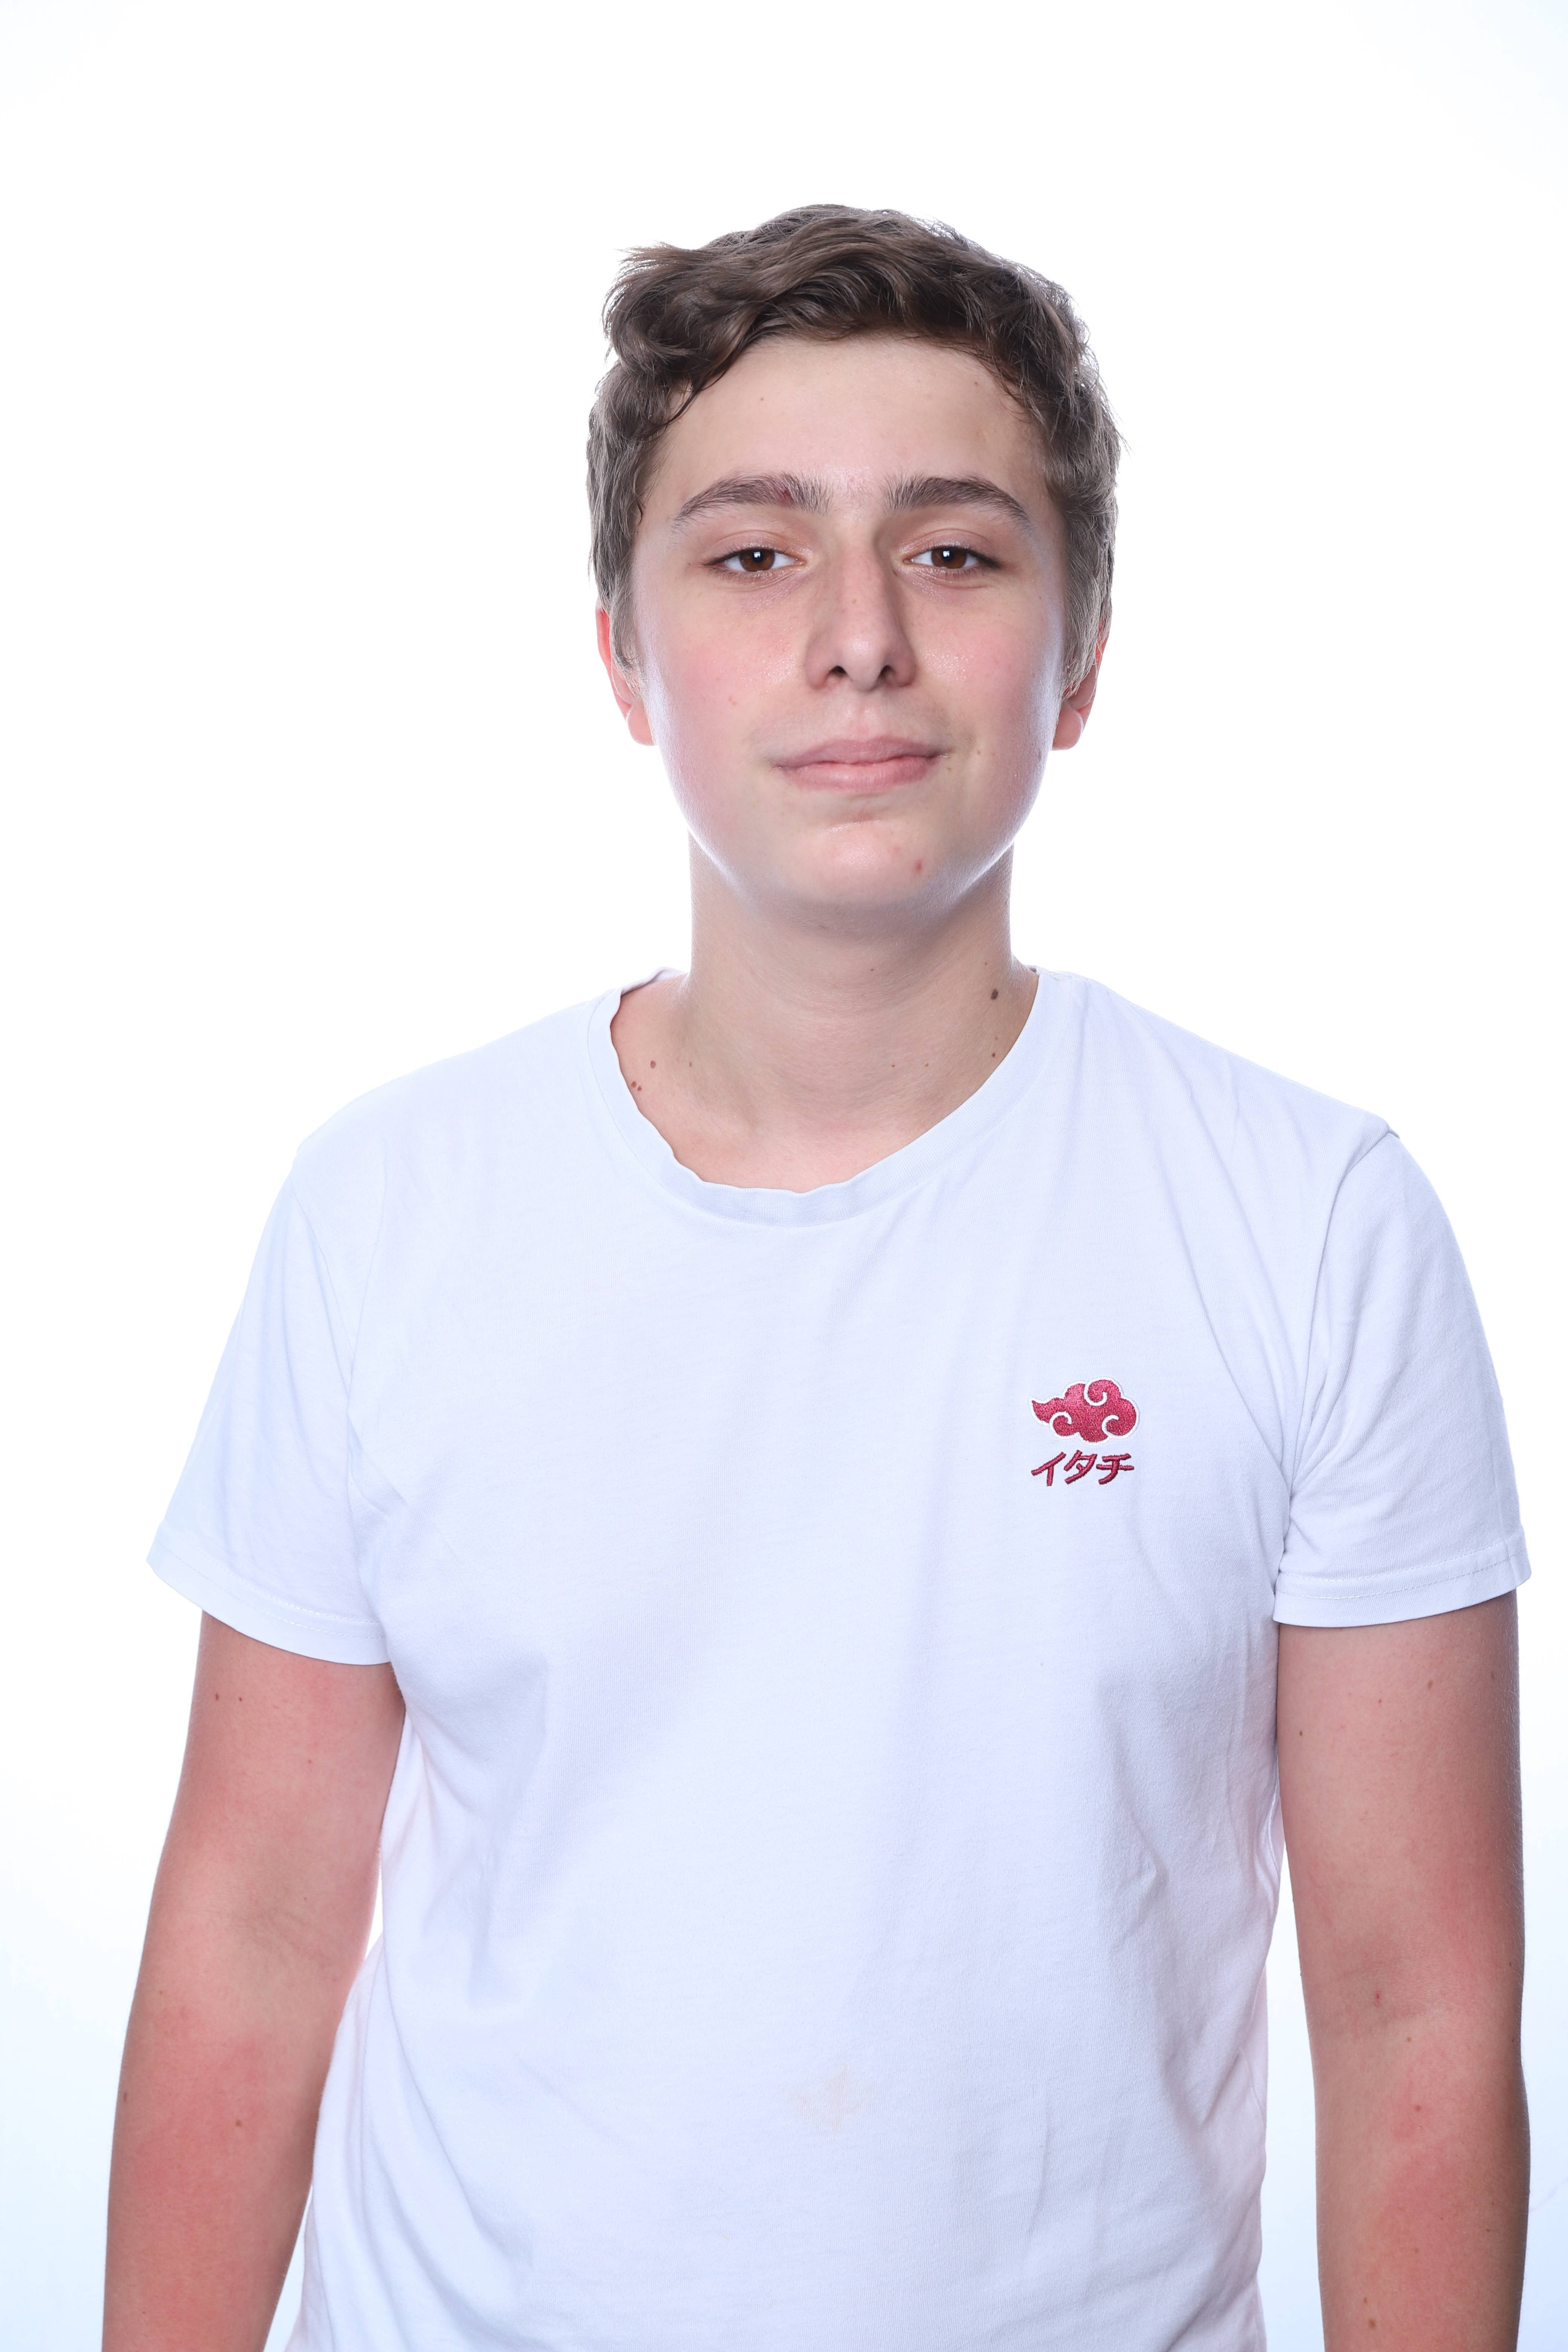
\includegraphics[scale=0.03]{images/josselin.priet.jpg}}
Josselin Priet, 17 ans, élève à EPITA, a commencé la programmation par Scratch et Unity. Au lycée, Josselin choisit les spécialités NSI, Mathématiques et HGGSP. Il a choisi cette dernière pour sa passion pour le journalisme. Durant son année de terminale, il a été à l’origine de 6 projets différents. Il est donc aussi passionné par la création de projets informatiques, que ce soit l’idée, l’algorithme, la partie code ou encore la partie débogage.

\noindent Dans ce projet, Josselin sera utile pour la partie algorithme, la conversion de concepts théoriques en programme et l'intelligence artificielle.
\clearpage


Guillaume Rat, actuellement élève à Epita, a \InsertBoxR{0}{
\includegraphics[scale=0.25]{images/guillaume.rat.jpg}}\noindent suivi les spécialités Mathématiques, Physique et NSI durant le lycée. Il est passionné par la programmation et l’informatique en général, cela vient en partie de son père. Il en apprend sur l’informatique en le regardant travailler sur des réseaux informatiques. L’idée de créer un projet de 0 et de le voir complété est un bel objectif qu'il a toujours voulu réaliser mais par manque de moyens et de temps il n'en a pas encore eu l'occasion. C’est pourquoi il est impatient de pouvoir commencer à travailler sur ce projet.

\noindent Durant ce projet, Guillaume sera utile pour le stockage des données, la gestion de réseau du jeu mais aussi la création du site internet.

\InsertBoxL{0}{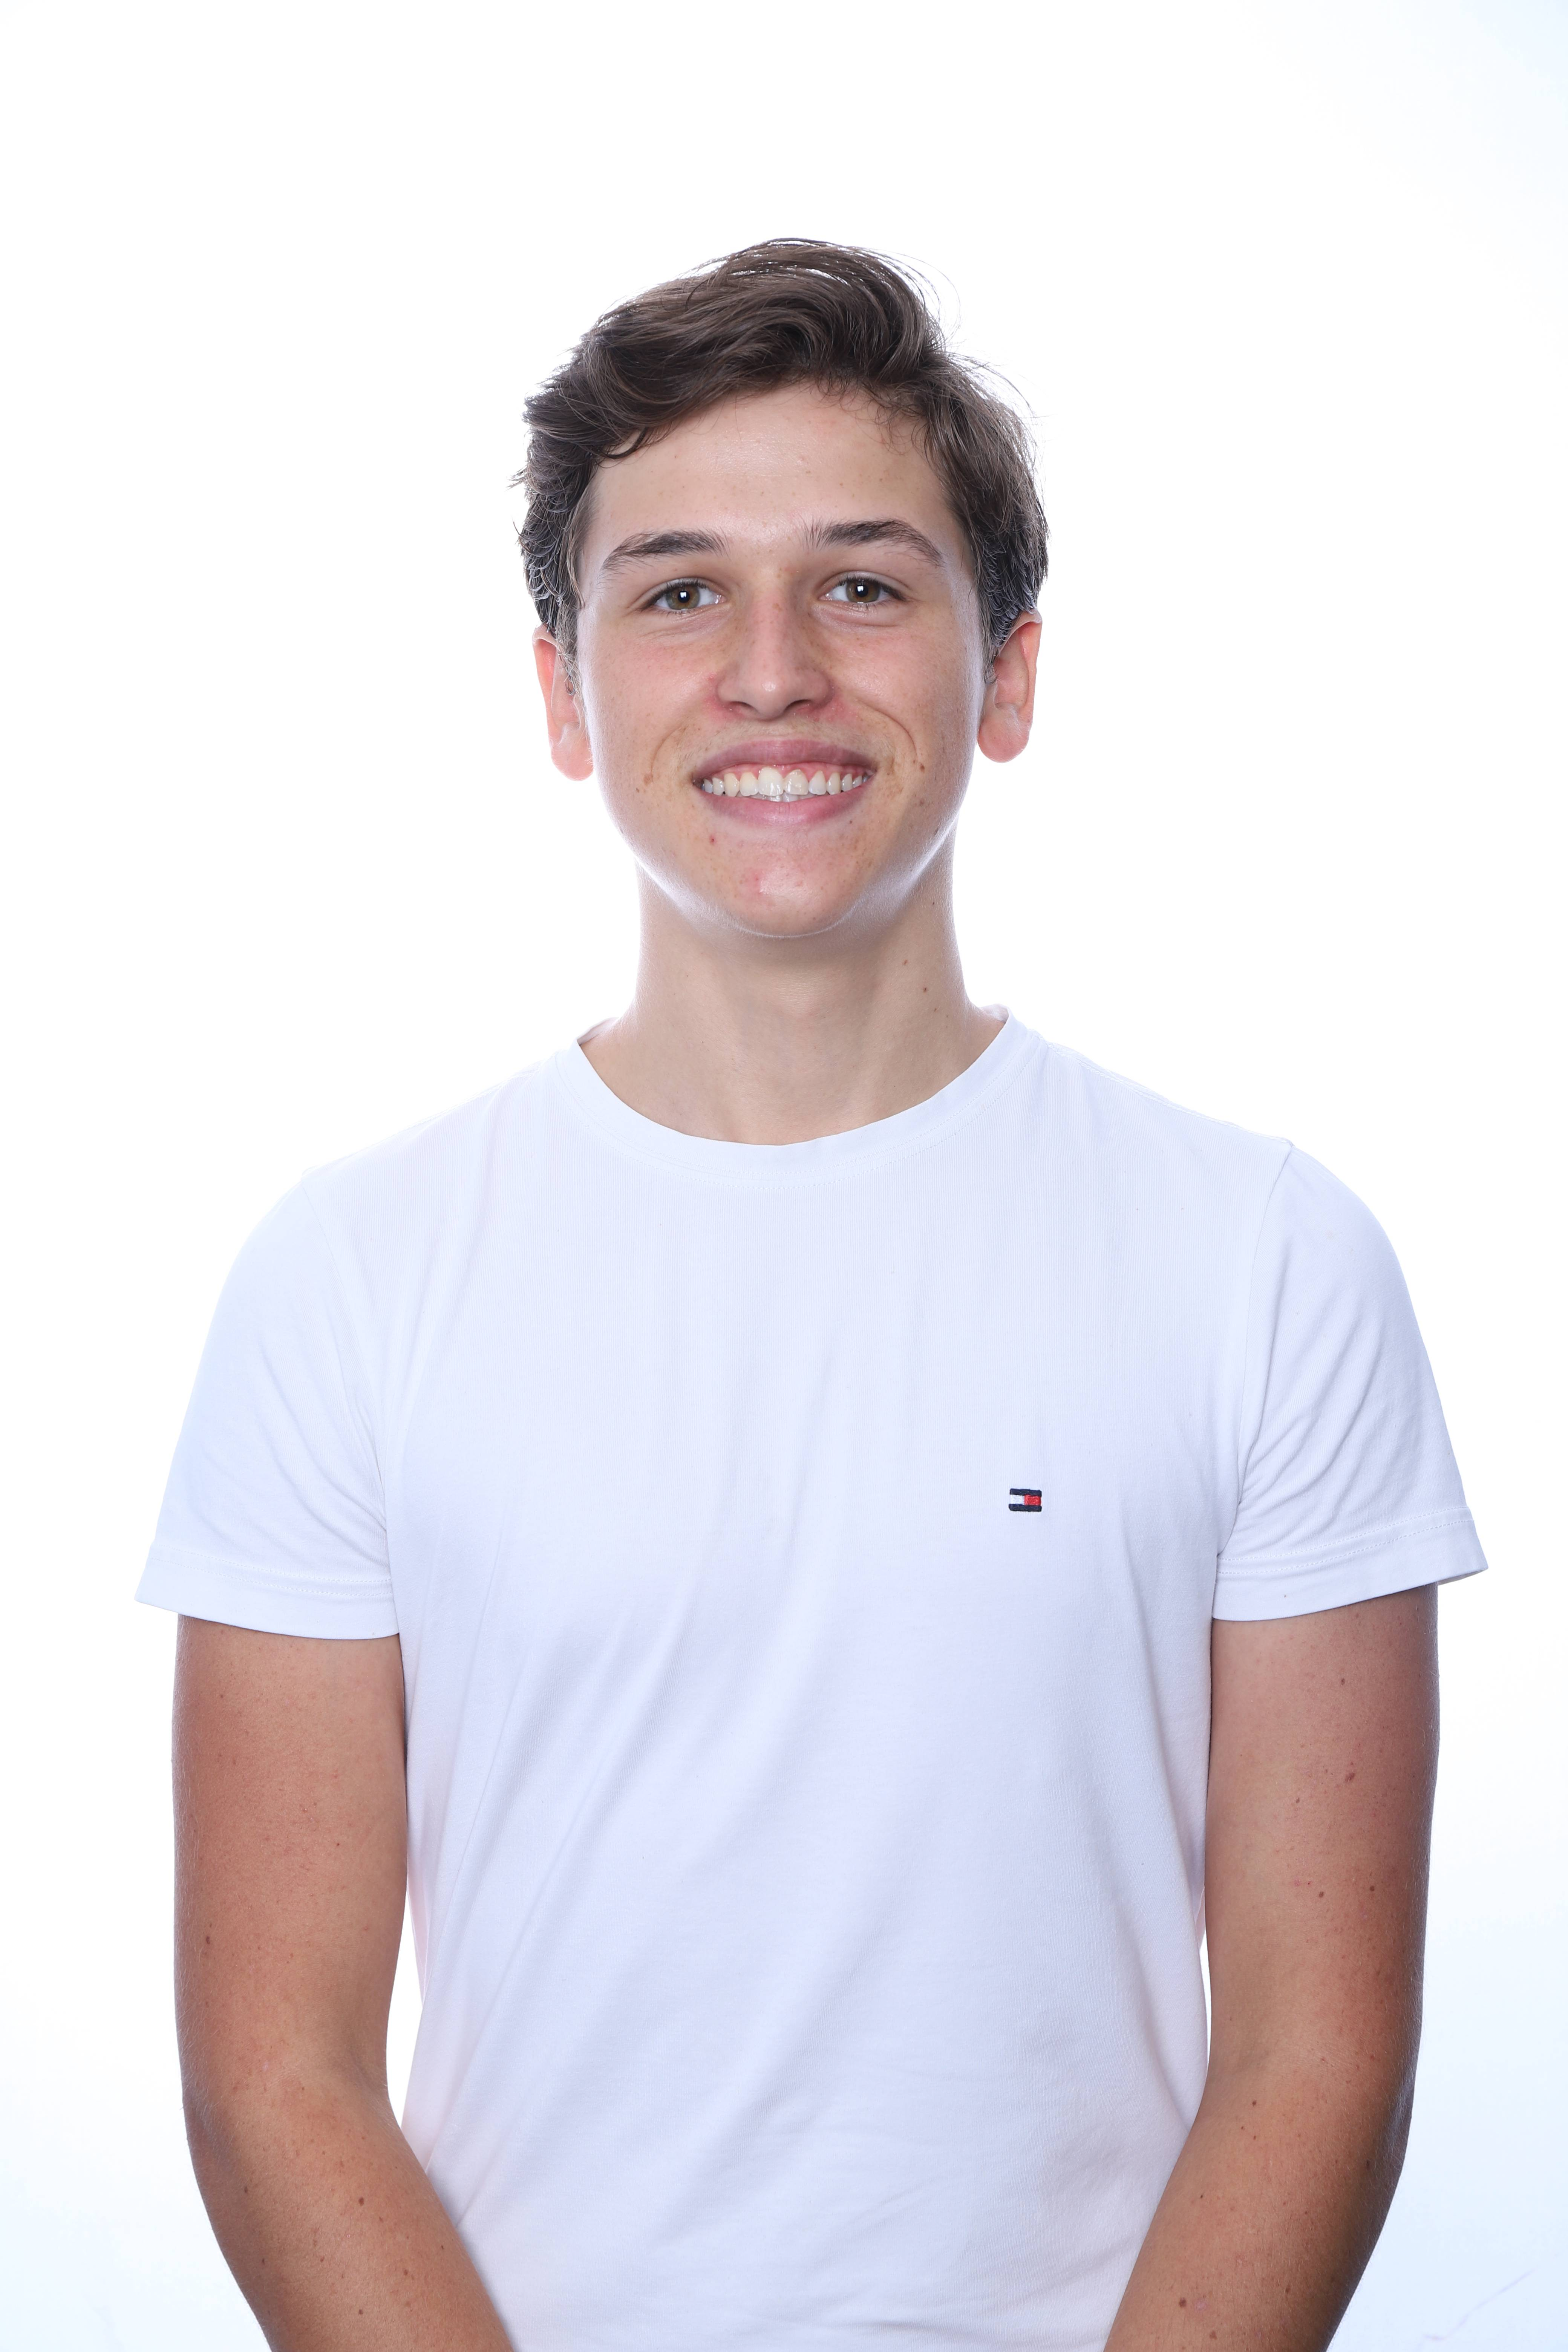
\includegraphics[scale=0.03]{images/hector.thubert.jpg}}
Hector Thubert, 18 ans, actuellement élève à Epita, passionné par la robotique, crée ses premiers robots grâce à des modules Arduino. Il a également créé plusieurs jeux vidéo dans différents langages durant ses années de lycée. Il choisit ainsi les spécialités Mathématiques, Physique et NSI. Cette dernière lui a permis de développer des compétences de programmation en Python et d’approfondir ses connaissances en informatique. Étant très curieux, cela l’aide à développer son sens de l’autonomie et son esprit d’initiative.

\noindent Dans ce projet, Hector sera utile pour créer la dynamique au sein du groupe, pour la partie graphisme mais aussi pour la création du site internet.
\clearpage


Guilhem Dardonville, actuellement élève à \InsertBoxR{0}{\includegraphics[scale=0.03]{images/guilhem.dardonville.png}}\noindent Epita, a suivi les spécialités NSI, Mathématiques et Physique au cours du lycée. Ces spécialités lui ont permis d'en découvrir davantage sur le monde actuel et son fonctionnement. Pour lui, les travaux de groupe sont importants pour la cohésion d'équipe et la répartition des tâches. C'est pourquoi, réaliser un projet de 0 est une expérience très intéressante et remplie de surprises qui ne peuvent qu'apporter du bien à la maturité du groupe.

\noindent Dans ce projet, Guilhem sera utile pour développer la physique du jeu, mais aussi pour la partie algorithmique et l'implémentation des concepts dans le jeu.
\clearpage

\subsection{Répartition des tâches}
\textit{(Prévision approximative)}

\begin{tabular}{|*6{c|}}
\hline
\diagbox{$Tâche$}{$Poste$} & Adrien & Josselin & Guillaume & Hector & Guilhem\\
\hline
Cahier des charges & R & S & S & S & S\\
\hline
Site internet &  &  & S & R & \\
\hline
Algorithme &  & R &  &  & S\\
\hline
Architecture de base & R & S &  &  & \\
\hline
Graphismes & R &  &  & S & \\
\hline
Son/Musique & R & S &  &  & \\
\hline
Physique & S &  &  &  & R\\
\hline
Réseau/Serveurs &  &  & R &  & S\\
\hline
Stockage des données &  &  & R &  & S\\
\hline
Envoi des données &  & S & R &  & \\
\hline
Intelligence artificielle &  & R &  &  & S\\
\hline
Équilibrage & S & R &  &  & \\
\hline
Menu & S &  &  & R & \\
\hline
Implémentation &  & R &  &  & S\\
\hline
Programmation & R & R & R & R & R\\
\hline
\end{tabular}
\newline

R = Responsable

S = Suppléant

\clearpage

\subsection{Avancement et planification}
\textit{(Prévision approximative)}

\begin{tabular}{|*4{c|}}
\hline
\diagbox{$Tâche$}{$Soutenance$} & 22 janvier (1) & 18 mars (2) & 17 juin (3)\\
\hline
Cahier des charges & 90\% & 95\% & 100\%\\
\hline
Site internet & 60\% & 80\% & 100\%\\
\hline
Algorithme & 100\% & 100\% & 100\%\\
\hline
Architecture de base & 100\% & 100\% & 100\%\\
\hline
Graphismes & 40\% & 70\% & 100\%\\
\hline
Son/Musique & 60\% & 80\% & 100\%\\
\hline
Physique & 20\% & 60\% & 100\%\\
\hline
Réseau/Serveurs & 30\% & 50\% & 100\%\\
\hline
Stockage des données & 10\% & 50\% & 100\%\\
\hline
Envoi des données & 60\% & 80\% & 100\%\\
\hline
Intelligence artificielle & 60\% & 80\% & 100\%\\
\hline
Équilibrage & 10\% & 40\% & 100\%\\
\hline
Menu & 20\% & 50\% & 100\%\\
\hline
Implémentation & 20\% & 60\% & 100\%\\
\hline
Programmation & 40\% & 70\% & 100\%\\
\hline
\end{tabular}
\newline
\newline
\clearpage


\newcommand\invisiblesection[1]{%
  \refstepcounter{section}%
  \addcontentsline{toc}{section}{\protect\numberline{\thesection}#1}%
  \sectionmark{#1}}

\invisiblesection{Cahier des charges technique}
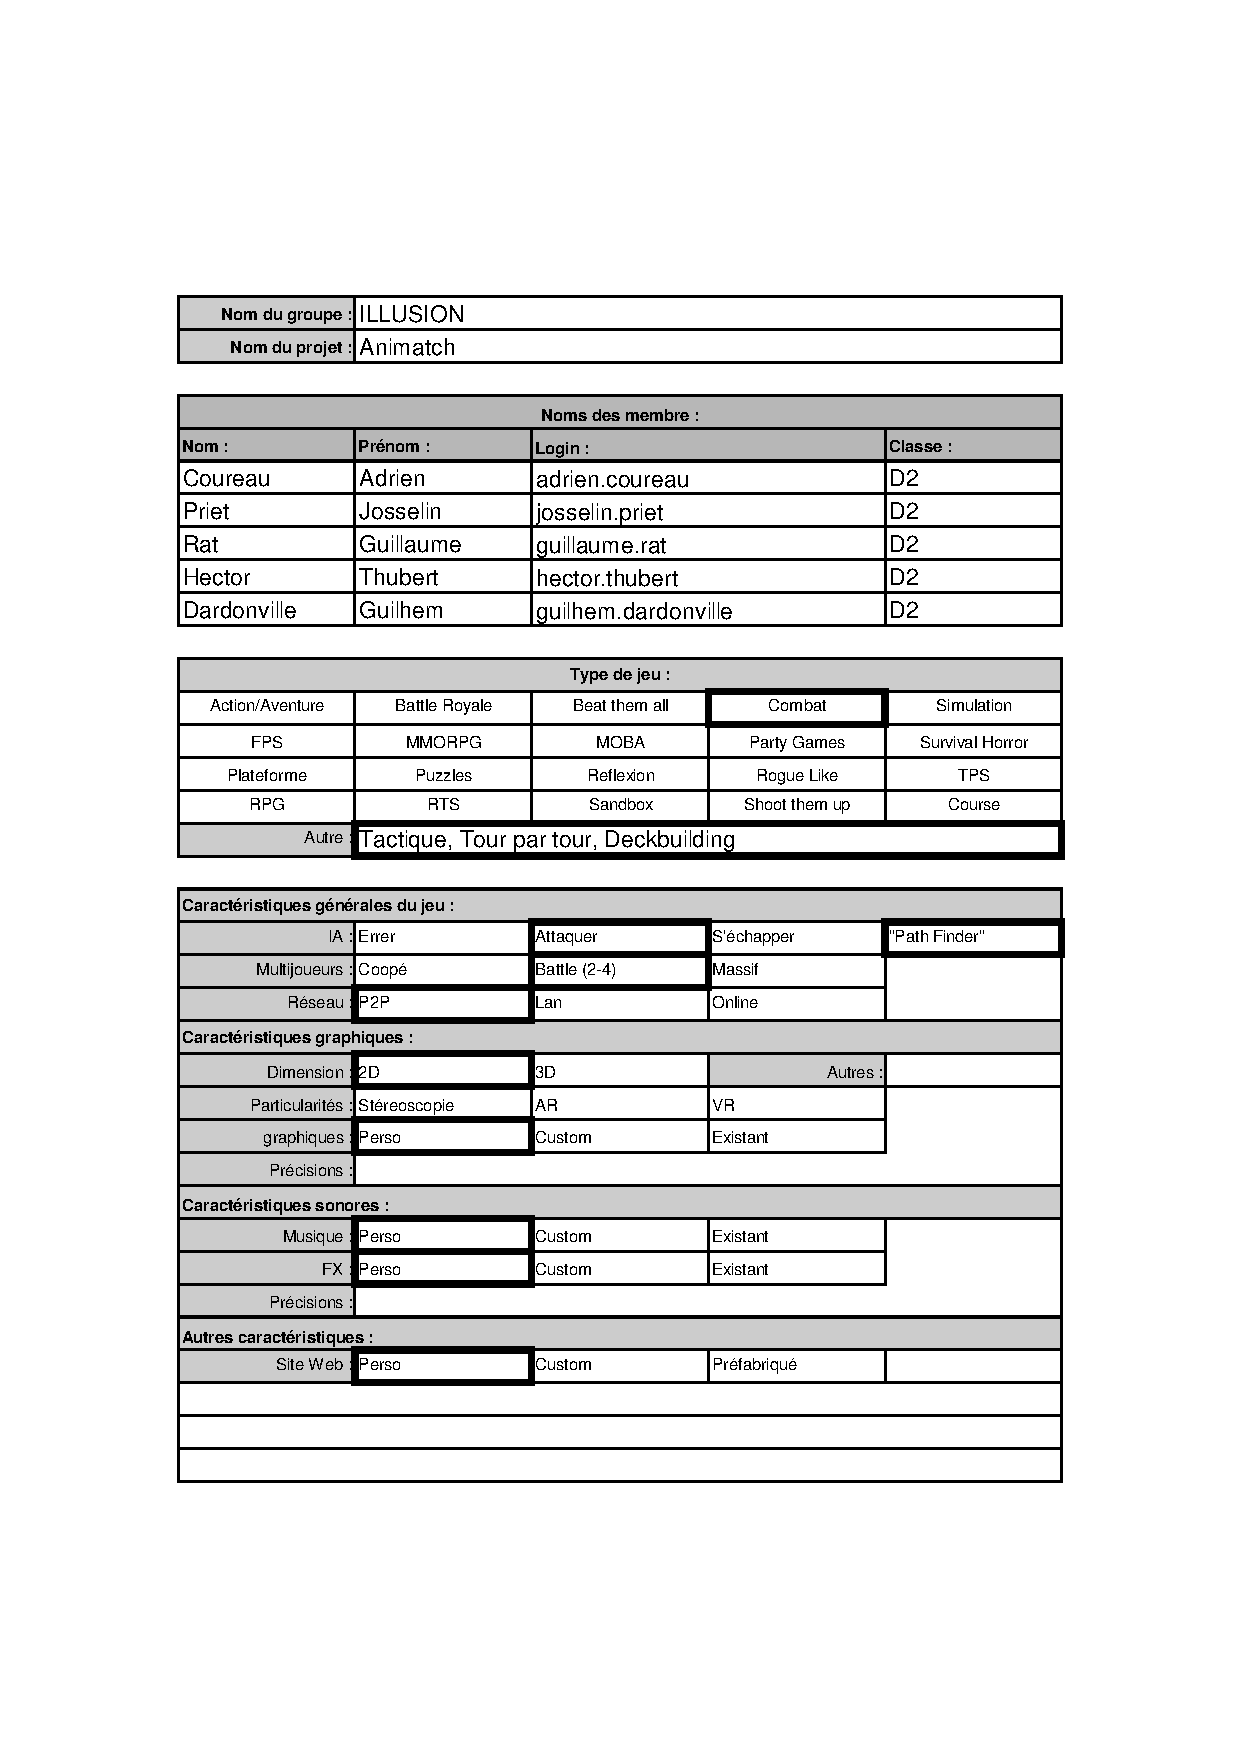
\includepdf[pages=-,fitpaper,
            pagecommand={\thispagestyle{plain}}
           ]{Cahier des charges technique.pdf}


\section{Conclusion}

Ainsi, Animatch est un projet de jeu vidéo mené par l'entreprise ILLUSION. Ce jeu allie des éléments de jeux de cartes et de combat en 2D sur un terrain destructible, conçu pour Windows avec une possible extension vers Android et iOS. L'objectif est de fournir un divertissement amusant pour les joueurs et d'enrichir les compétences et connaissances en informatique de l'équipe.
 
Le cahier des charges guidera le développement en définissant les concepts, les objectifs, les contraintes temporelles et budgétaires. Inspiré par \textit{Worms} et \textit{Clash Royale}, Animatch promet une expérience immersive en multijoueur ou en solo contre une intelligence artificielle.

L'entreprise ILLUSION est déterminée à réussir ce premier projet et compte sur l'engagement et les compétences de chaque membre de son équipe. Elle se spécialise dans le développement de jeux vidéo en utilisant des outils tels que Notion, Discord, et le moteur de jeu Godot.

Le projet Animatch est un défi passionnant pour l’entreprise, et nous sommes convaincus que le résultat final sera un jeu divertissant et innovant. Nous sommes impatients de voir ce projet prendre forme et de le présenter au public. Ce cahier des charges servira de guide tout au long du processus de développement.


\clearpage

\pagenumbering{arabic}
\end{document}
